%Jennifer Pan, August 2011

\documentclass[10pt,letter]{article}
	% basic article document class
	% use percent signs to make comments to yourself -- they will not show up.

\usepackage{amsmath}
\usepackage{amssymb}
	% packages that allow mathematical formatting

\usepackage{graphicx}
	% package that allows you to include graphics

\usepackage{setspace}
	% package that allows you to change spacing

\onehalfspacing
	% text become 1.5 spaced

\usepackage{fullpage}
	% package that specifies normal margins

\renewcommand{\vector}[1]{\boldsymbol{#1}}
\newcommand{\problem}[1]{\section*{Problem #1}}
\newcommand{\problempart}[1]{\paragraph{#1}}

\begin{document}
	% line of code telling latex that your document is beginning


\title{Problem Set 2}

\author{Nicholas Wu}

\date{Fall 2020}
	% Note: when you omit this command, the current dateis automatically included

\maketitle
	% tells latex to follow your header (e.g., title, author) commands.
\textbf{Note:} I use bold symbols to denote vectors and nonbolded symbols to denote scalars. I primarily use vector notation to shorthand some of the sums, since many of the sums are dot products.

\problem{1}

\problempart{(1)} The consumer's problem is given by:
\[ \max \sum_{t=0}^\infty \beta^t \log c_t\]
subject to
\[ c_t - b_{t+1} + k_{t+1} - (1-\delta) k_t \le r_t^k k_t + w_t - (1+r_t^b )b_t \]
\[ b_0 = 0 \]
\[ k_0 \le \bar{k}_0 \]
\[ c_t, k_t \ge 0 \]
\[ b_{t+1} \le B\]
where $B$ is the borrowing limit. We have to include a borrowing limit else a consumer can achieve any allocation they want by borrowing forward; i.e., for any $c^*$, we can set
\[ k_t = 0 \]
\[ b_1 =  c^*_0 - w_0 \]
\[ b_2 = ( c^*_1 - w_1) + (1+r_1^b)(w_0 - c^*_0)  \]
and so on
\[ b_{t+1} = c^*_t-w_t  + b_t(1 + r_t^b) \]
The form of $b_t$ is then
\[ b_t = \sum_{k=1}^{t} ( c^*_{k-1}-w_{k-1} ) \prod_{i={k}}^{t-1} (1+r_{i}^b) \]
The consumer is borrowing infinitely against the future, so the borrowing limit prevents these outcomes. Using the FOCs derived in lecture, the Euler conditions are given by
\[ \frac{1}{c_t} = \beta (1-\delta + r^k_{t+1})\frac{1}{c_{t+1}} \]
\[ c_{t+1} = c_t \beta (1-\delta + r^k_{t+1}) \]
\[ \frac{1}{c_t} = \beta (1 + r^b_{t+1})\frac{1}{c_{t+1}} \]
\[ c_{t+1} = c_t \beta (1 + r^b_{t+1}) \]
and the transversality conditions are given by
\[ \lim_{t \to \infty} \beta^t\frac{(1 + r^b_t) b_t}{c_t} = 0 \]
\[ \lim_{t \to \infty} \beta^t\frac{(1 - \delta + r^k_t) k_t}{c_t} = 0 \]

\problempart{(2)}
The sequential equilibrium given initial savings and capital $\bar{b}_0$, $\bar{k}_0$ consists of a consumer allocation $\{ (c_t, k_t, b_t) \}_{t=0}^\infty$, a producer allocation $\{ k_t^f, l_t^f \}_{t=0}^\infty$, and prices/wages $\{ w_t, r_t^b, r_t^k \}_{t=0}^\infty$, that satisfy the following conditions:
\begin{itemize}
\item The consumer alllocation solves the consumer maximization problem for the given $\bar{b}_0$, $\bar{k}_0$, $\{ w_t, r_t^b, r_t^k \}_{t=0}^\infty$. We stated the problem in the previous part, but here it is again:
\[ \max \sum_{t=0}^\infty \beta^t \log c_t\]
subject to
\[ c_t - b_{t+1} + k_{t+1} - (1-\delta) k_t \le r_t^k k_t + w_t - (1+r_t^b )b_t \]
\[ b_0 = \bar{b}_0, \ k_0 \le \bar{k}_0 \]
\[ c_t, k_t \ge 0, \ b_{t+1} \ge -B\]
\item The producer allocation maximizes profits for the firm, or $(k_t^f, l_t^f)$ maximizes:
\[ \max F(k_t^f, l_t^f) - r_t^k k_t^f - w_tl_t^f\]
subject to
\[ k_t^f, l_t^f \ge 0 \]
\item All markets clear:
\[ k_t = k_t^f \]
\[ l_t^f = 1 \]
\[ b_t = 0 \]
\[ c_t + k_{t+1} - (1-\delta) k_t = F(k_t^f, l_t^f) \]
\end{itemize}
In terms of relating the interest rates, we have the no-arbitrage condition, that
\[ 1-\delta +r^k_{t+1} = 1+ r^b_{t+1}\]
\[ r^k_{t+1} - \delta = r^b_{t+1}\]
Intuitively, this makes sense; if a consumer can achieve higher returns by investing in bonds rather than in capital, they would invest no capital, and no production could occur. Conversely, if a consumer can achieve higher returns in capital rather than bonds, the consumer would then choose to always borrow using bonds to buy capital, and will guarantee a profit, which violates the equilibrium assumption of $b_t = 0$.
\problempart{(3)} In this case, an allocation is governed by $\{ k_t^f, c_t, l_t^f \}$, and our feasibility constraints are:
\[ k_0^f \le \bar{k}_0 \]
\[ c_t \ge 0, \ k_t^f \ge 0, \ l_t^f \in [0,1] \]
\[ c_t \le F(k_t^f, l_t^f) + (1-\delta)k_t^f - k_{t+1}^f \]
\problempart{(4)} An Arrow-Debreu equilibrium consists of allocation $\{ k_t^f, c_t, l_t^f \}$, wages/good prices $\{ w_t, p_t \}$, and an initial price of capital $p^k$ such that:
\begin{itemize}
\item The consumer maximizes utility subject to his/her budget constraint. That is, the consumer allocation $\{ c_t \}$ is a maximizer for:
\[ \max \sum_{t=0}^\infty \beta^t \log c_t  \]
subject to
\[ \sum_{t=0}^\infty p_t c_t \le p_0 p^k \bar{k}_0 + \sum_{t=0}^\infty p_t w_t \]
\[ c_t \ge 0\]
\item The producer maximizes profits. This means $\{ k_t^f, l_t^f \}$ maximizes:
\[ \max \left(-p_0 p^k \bar{k}_0 + \sum_{t=0}^\infty p_t F(k_t^f, l_t^f) - p_tw_tl_t^f - p_tk^f_{t+1} + p_t(1-\delta)k^f_t \right) \]
subject to
\[ k^f_t\ge 0, \ l^f_t \ge 0  \]
\item Markets clear. That is,
\[ c_t + k^f_{t+1} = F(k^f_t, l^f_t) \]
\[ l_t^f = 1 \]
\[ k^f_0 = \bar{k}_0 \]
\end{itemize}
\problempart{(5)}
In this case, an equilibrium consists of firm allocation $\{ k_t^f, l_t^f \}$, consumer allocation $\{ c_t, k_t \}$, prices $\{ p_t \}$, wages $\{ w_t \}$, and rental rate $\{ r_t \}$. The equilibrium must satisfy:
\begin{itemize}
\item Consumers maximize their own utility: that is, $\{c_t, k_t \}$ is an optimizer of
\[ \max \sum_{t=0}^\infty \beta^t \log c_t \]
subject to
\[ \sum_{t=0}^\infty p_t c_t + \sum_{t=0}^\infty p_t (k_{t+1} - (1-\delta)k_t)  \le \sum_{t=0}^\infty (p_t w_t + p_t r_t k_t) \]
\[ c_t\ge 0, \ k_t \ge 0 \]
\item Firms maximize profits: that is, $k_t^f, l_t^f$ maximizes
\[ \max p_t (F(k^f_t, l^f_t) - w_t l^f_t -r_t k^f_t) \]
subject to
\[k^f_t \ge 0, \ l^f_t \ge 0\]
\item Markets clear:
\[ k_t = k^f_t \]
\[ l_t^f = 1 \]
\[ c_t + k_{t+1}^f = F(k^f_t, l^f_t) \]
\[ k_0 = \bar{k}_0 \]
\end{itemize}
\problempart{(6)}
Intuitively, since the FWT gives that these problems are equivalent to the social planner problem, we know the allocations are all the same across the different equilibria. Specifically:
\begin{itemize}
\item $(2) \to (4)$: We first see that to preserve firm optimization behavior, we set wages equal between the two problems. Then we need to nail down the prices. The firm's objective in $(2)$ is:
\[ F(k_t^f, l_t^f) - r_t^k k_t^f - w_tl_t^f \]
Note that this objective can be multiplied by a scalar and still preserve the optimization behavior. Now, consider the firm's objective in $(4)$:
\[-p_0 p^k \bar{k}_0 + \sum_{t=0}^\infty p_t F(k_t^f, l_t^f) - p_tw_tl_t^f - p_tk^f_{t+1} + p_t(1-\delta)k^f_t \]
Isolating the terms, we see for $t \ge 1$ the terms are:
\[p_t F(k_t^f, l_t^f) - p_tw_tl_t^f - p_{t-1}k^f_{t} + p_t(1-\delta)k^f_t\]
We want this to be equivalent to the objective in $(2)$, so we let this equal the objective of $(2)$ multiplied by the scalar $p_t$:
\[ p_t(F(k_t^f, l_t^f) - r_t^k k_t^f - w_tl_t^f) = p_t F(k_t^f, l_t^f) - p_tw_tl_t^f - p_{t-1}k^f_{t} + p_t(1-\delta)k^f_t \]
\[ -p_tr_t^kk_t^f = - p_{t-1}k_t^f + p_t(1-\delta)k^f_t \]
\[ r_t^k = \frac{p_{t-1}}{p_t} - (1-\delta) \]
\[ p_t = \frac{p_{t-1}}{1 - \delta + r_t^k} \]
So we get the prices can be found by normalizing $p_0$, and using this identity:
\[ p_0 = p^* \]
\[ p_t = p^* \prod_{t=0}^{t-1} \frac{1}{1-\delta + r_{t+1}^k}\]
For the initial capital price, we take the same approach as for finding prices, but we investigate the terms of the corresponding firm objectives with $t=0$.
\[ p_0(F(k_0^f, l_0^f) - r_0^k k_0^f - w_0l_0^f) = p_0 F(k_0^f, l_0^f) - p_0w_0l_0^f - p_0 p^k k^f_{0} + p_0(1-\delta)k^f_0 \]
\[ - r_0^k  =  - p^k + (1-\delta) \]
\[ p^k = r_0^k + (1-\delta) \]
So we get the following result:

\textbf{Theorem}: Suppose we have a consumer allocation $\{ (c_t, k_t, b_t) \}_{t=0}^\infty$, a producer allocation $\{ k_t^f, l_t^f \}_{t=0}^\infty$, and wages/rates $\{ w_t, r_t^b, r_t^k \}_{t=0}^\infty$ that is an equilibrium for the market given in $(2)$. Then the same allocation $\{ c_t \}_{t=0}^\infty$  with $\{ k_t^f, l_t^f \}_{t=0}^\infty$ is supported as an equilibrium in $(4)$ with prices given by:
\begin{itemize}
\item Wage rate: $w'_t = w_t$
\item Prices:
\[ p_0 = p^* \]
\[ p_t = p^* \prod_{t=1}^{t} \frac{1}{1-\delta + r_{t}^k}\]
\item Initial capital price:
\[ p^k = r_0^k + (1-\delta) \]
\end{itemize}
\item $(2) \to (5)$: We note that $(5)$ is the standard Arrow-Debreu counterpart of the sequential equilibrium problem in $(2)$. Thus, we have the following:

\textbf{Theorem}: Suppose we have a consumer allocation $\{ (c_t, k_t, b_t) \}_{t=0}^\infty$, a producer allocation $\{ k_t^f, l_t^f \}_{t=0}^\infty$, and wages/rates $\{ w_t, r_t^b, r_t^k \}_{t=0}^\infty$ that is an equilibrium for the market given in $(2)$. Then the same allocation $\{ c_t, k_t \}_{t=0}^\infty$  with $\{ k_t^f, l_t^f \}_{t=0}^\infty$ is supported as an equilibrium in $(5)$ with prices given by:
\begin{itemize}
\item Wage rate: $w'_t = w_t$
\item Capital rental rate: $r'_t = r^k_t$
\item Prices:
\[ p_0 = p^* \]
\[ p_t = p^* \prod_{t=1}^{t} \frac{1}{1-\delta + r_{t}^k}\]
\end{itemize}
\item $(4) \to (2)$: We have the same equivalences as our theorem from $(2) \to (4)$. That is, for $t \ge 1$, we have
\[ r_t^k = \frac{p_{t-1}}{p_t} - (1-\delta) \]
And for $t = 0$:
\[ p^k = r_0^k + (1-\delta) \]
\[ r_0^k = p^k - (1-\delta)\]

\textbf{Theorem}: Suppose we have an equilibrium for $(4)$ with alllocation $\{ k_t^f, c_t, l_t^f \}_{t=0}^\infty$, wages/good prices $\{ w_t, p_t \}$, and an initial price of capital $p^k$. Then the consumer allocation $\{ c_t, k_t = k_t^f, b_t = 0 \}_{t=0}^\infty$ and producer allocation $\{ k_t^f, l_t^f \}_{t=0}^\infty$ is supported as a sequential equilibrium in $(2)$ with prices:
\begin{itemize}
\item Wage rate: $w'_t = w_t$
\item Capital rental rate:
\[ r_0^k = p^k - (1-\delta)\]
and for $t \ge 1$:
\[ r_t^k = \frac{p_{t-1}}{p_t} - (1-\delta) \]
\item Bond rental rate: $r^b_t = r^k_t - \delta$
\end{itemize}
\item $(4) \to (5)$: We match the firm problems in these two equilibriums in order to support the same allocation. The firm's objective to maximize in $(5)$ is
\[ p_t F(k_t^f, l_t^f) - p_t w_t l_t^f - p_t r^k_t k_t^f \]
In $(4)$ the firm's objective is
\[ -p_0 p^k \bar{k}_0 + \sum_{t=0}^\infty p_t F(k_t^f, l_t^f) - p_tw_tl_t^f - p_tk^f_{t+1} + p_t(1-\delta)k^f_t  \]
Isolating the terms with $k_t^f, l_t^f$, we get for $t \ge 1$
\[ p_t F(k_t^f, l_t^f) - p_tw_tl_t^f - p_{t-1}k^f_{t} + p_t(1-\delta)k^f_t \]
and for $t=0$,
\[ p_0 F(k_0^f, l_0^f) - p_0w_0l_0^f - p_0 p^k \bar{k}_0 + p_0(1-\delta)k^f_0 \]
Setting this equal to the incentive constraint in $(5)$, we get
\[ p_t F(k_t^f, l_t^f) - p_t w_t l_t^f - p_t r^k_t k_t^f = p_t F(k_t^f, l_t^f) - p_tw_tl_t^f - p_{t-1}k^f_{t} + p_t(1-\delta)k^f_t \]
\[ - p_t r^k_t = - p_{t-1}+ p_t(1-\delta) \]
\[ r^k_t = \frac{p_{t-1}}{p_t} - (1-\delta) \]
for $t \ge 1$. At $t=0$, we have
\[ p_0 F(k_0^f, l_0^f) - p_0 w_0 l_0^f - p_0 r^k_0 k_0^f = p_0 F(k_0^f, l_0^f) - p_0w_0l_0^f - p_0 p^k \bar{k}_0 + p_0(1-\delta)k^f_0 \]
\[ r^k_0  = p^k  - (1-\delta) \]
So we have the result:

\textbf{Theorem}: Suppose we have an equilibrium for $(4)$ with alllocation $\{ k_t^f, c_t, l_t^f \}_{t=0}^\infty$, wages/good prices $\{ w_t, p_t \}$, and an initial price of capital $p^k$. Then the same allocation $\{ c_t, k_t = k_t^f \}_{t=0}^\infty$  with $\{ k_t^f, l_t^f \}_{t=0}^\infty$ is supported as an equilibrium in $(5)$ with prices given by:
\begin{itemize}
\item Wage rate: $w'_t = w_t$
\item Prices: $p'_t = p_t$
\item Capital rental rate:
\[ r^k_0  = p^k  - (1-\delta) \]
For $t \ge 1$,
\[ r^k_t = \frac{p_{t-1}}{p_t} - (1-\delta) \]
\end{itemize}
\item $(5) \to (2)$: This is the conventional Arrow-Debreu / sequential equilibrium equivalence. So we have:

\textbf{Theorem}: Suppose we haave an equilibrium for $(5)$ with allocation $\{ k_t^f, l_t^f \}_{t=0}^\infty$, consumer allocation $\{ c_t, k_t \}_{t=0}^\infty$, prices $\{ p_t \}_{t=0}^\infty$, wages $\{ w_t \}_{t=0}^\infty$, and capital rental rate $\{ r_t \}_{t=0}^\infty$. Then the consumer allocation $\{ c_t, k_t, b_t = 0 \}_{t=0}^\infty$ and producer allocation $\{ k_t^f, l_t^f \}_{t=0}^\infty$ is supported as a sequential equilibrium in $(2)$ with prices:
\begin{itemize}
\item Wage rate: $w'_t = w_t$
\item Capital rental rate: $r^k_t = r_t$
\item Bond rental rate: $r^b_t = r^k_t - \delta$
\end{itemize}
\item $(5) \to (4)$: As in the direction $(4) \to (5)$, we match the firm's problem. So we can match the same wages and prices, and we need to find the initial capital price:
\[ r^k_0  = p^k  - (1-\delta) \]
\[ p^k = r^k_0 + (1-\delta) \]

Suppose we haave an equilibrium for $(5)$ with allocation $\{ k_t^f, l_t^f \}_{t=0}^\infty$, consumer allocation $\{ c_t, k_t \}_{t=0}^\infty$, prices $\{ p_t \}_{t=0}^\infty$, wages $\{ w_t \}_{t=0}^\infty$, and rental rate $\{ r_t \}_{t=0}^\infty$. Then the same allocation $\{ c_t \}_{t=0}^\infty$  with $\{ k_t^f, l_t^f \}_{t=0}^\infty$ is supported as an equilibrium in $(4)$ with prices given by:
\begin{itemize}
\item Wage rate: $w'_t = w_t$
\item Prices: $p'_t = p_t$
\item Initial capital price:
\[ p^k = r^k_0 + (1-\delta) \]
\end{itemize}
\end{itemize}
\problem{2}
\problempart{(1)}
Using the constraint binding, we get
\[ c_t = \theta k_t^\alpha + (1-\delta)k_t - k_{t+1} \]
Then we can take:
\[ F(k_t, k_{t+1}) = \frac{(\theta k_t^\alpha + (1-\delta)k_t - k_{t+1})^{1-\sigma} - 1}{1-\sigma} \]
and
\[ \Gamma(k_t) = [0, \theta k_t^\alpha + (1-\delta)k_t]\]
The Lagrangian is given by
\[ \sum_{t=0}^\infty \beta^t F(k_t, k_{t+1}) - \lambda_t k_t \]
The FOCs are:
\[ \beta^{t+1} F_1(k_{t+1}, k_{t+2}) + \beta^t F_2(k_{t}, k_{t+1})  = \lambda_{t+1} \]
\[ \beta F_1(k_{t+1}, k_{t+2}) + F_2(k_{t}, k_{t+1})  = 0 \]
The Euler condition is
\[ \frac{1}{(\theta k_t^\alpha + (1-\delta)k_t - k_{t+1})^\sigma} = \frac{\beta(1-\delta + \alpha \theta k_t^{\alpha - 1})}{(\theta k_{t+1}^\alpha + (1-\delta)k_{t+1} - k_{t+2})^\sigma} \]
\[ \theta k_{t+1}^\alpha + (1-\delta)k_{t+1} - k_{t+2} = (\theta k_t^\alpha + (1-\delta)k_t - k_{t+1}) \beta^{1/\sigma}(1-\delta + \alpha \theta k_t^{\alpha - 1})^{1/\sigma} \]
The transversality condition is
\[ \lim_{t\to\infty} \frac{\beta^t \left( \theta \alpha k_t^{\alpha} + (1 - \delta)k_t \right)}{(\theta k_t^\alpha + (1-\delta)k_t - k_{t+1})^{\sigma}}  = 0 \]
\problempart{(2)} Suppose the sequence $\{ k_t \}_{t=0}^\infty$ satisfies the Euler condition and transversality condition. To show $\{ k_t \}_{t=0}^\infty$ indeed optimizes the objective, consider some other feasible $\{ k_t' \}_{t=0}^\infty$. We claim
\[ \Delta = \sum_{t=0}^\infty \beta^T F(k_t) - \sum_{t=0}^\infty \beta^T F(k'_t) \ge 0 \]
Using the fact that $F$ is concave, continuous, and differentiable, we have
\[ F(k_t, k_{t+1}) - F(k'_t, k'_{t+1}) \ge F_1(k_t, k_{t+1})(k_t - k'_t) + F_2(k_t, k_{t+1})(k_{t+1} - k'_{t+1})  \]
Multiplying both sides by $\beta^t$, we get
\[ \Delta = \lim_{T \to \infty} \left( \sum_{t=0}^T\beta^t(F(k_t, k_{t+1}) - F(k'_t, k'_{t+1})) \right)  \]
\[\ge \lim_{T \to \infty} \left( \sum_{t=0}^T\beta^t(F_1(k_t, k_{t+1})(k_t - k'_t) + F_2(k_t, k_{t+1})(k_{t+1} - k'_{t+1})) \right)  \]
\[=\lim_{T \to \infty} \left( \sum_{t=0}^T\beta^t F_1(k_t, k_{t+1})(k_t - k'_t) + \sum_{t=0}^T\beta^t F_2(k_t, k_{t+1})(k_{t+1} - k'_{t+1}) \right)  \]
\[=\lim_{T \to \infty} \left( \sum_{t=0}^T\beta^t F_1(k_t, k_{t+1})(k_t - k'_t) + \sum_{t=0}^{T-1}\beta^t F_2(k_t, k_{t+1})(k_{t+1} - k'_{t+1}) + \beta^T F_2(k_T, k_{T+1})(k_{T+1} - k'_{T+1}) \right)  \]
Note $k_0 = k'_0$, so we have
\[\Delta \ge \lim_{T \to \infty} \left( \sum_{t=0}^T\beta^t F_1(k_t, k_{t+1})(k_t - k'_t) + \sum_{t=0}^{T-1}\beta^t F_2(k_t, k_{t+1})(k_{t+1} - k'_{t+1}) + \beta^T F_2(k_T, k_{T+1})(k_{T+1} - k'_{T+1}) \right)  \]
\[ = \lim_{T \to \infty} \left( \sum_{t=1}^T\beta^t F_1(k_t, k_{t+1})(k_t - k'_t) + \sum_{t=0}^{T-1}\beta^t F_2(k_t, k_{t+1})(k_{t+1} - k'_{t+1}) + \beta^T F_2(k_T, k_{T+1})(k_{T+1} - k'_{T+1}) \right)  \]
\[ = \lim_{T \to \infty} \left( \sum_{t=0}^{T-1}\beta^{t+1} F_1(k_{t+1}, k_{t+2})(k_{t+1} - k'_{t+1}) + \sum_{t=0}^{T-1}\beta^t F_2(k_t, k_{t+1})(k_{t+1} - k'_{t+1}) + \beta^T F_2(k_T, k_{T+1})(k_{T+1} - k'_{T+1}) \right)  \]
\[ = \lim_{T \to \infty} \left( \sum_{t=0}^{T-1}\beta^{t} \left( \beta F_1(k_{t+1}, k_{t+2})+ F_2(k_t, k_{t+1})\right)(k_{t+1} - k'_{t+1}) + \beta^T F_2(k_T, k_{T+1})(k_{T+1} - k'_{T+1}) \right)  \]
By the Euler condition, the sum is 0 (because the summand is 0), so
\[ \Delta \ge \lim_{T \to \infty} \left(\beta^T F_2(k_T, k_{T+1})(k_{T+1} - k'_{T+1}) \right)  \]
Also by the Euler condition, $ F_2(k_T, k_{T+1}) = - \beta F_1(k_{T+1}, k_{T+2})$, so this becomes
\[ \Delta \ge \lim_{T \to \infty} \left(- \beta^{T+1} F_1(k_{T+1}, k_{T+2})(k_{T+1} - k'_{T+1}) \right)  \]
\[ \Delta \ge \lim_{T \to \infty} \left(\beta^{T+1} F_1(k_{T+1}, k_{T+2})(k'_{T+1} - k_{T+1}) \right)  \]
Since $k'_{T+1}$ is nonnegative,
\[ \Delta \ge -\lim_{T \to \infty} \left(\beta^{T+1} F_1(k_{T+1}, k_{T+2}) k_{T+1} \right) \]
But by transversality condition, the limit on the RHS is 0, so $\Delta \ge 0$. Hence $\{ k_t \}_{t=0}^\infty$ is optimal.

\problempart{(3)} If we examine the original social planner problem, we see that the budget constraint must bind: if not, we can allocate more $c_t$ for some period, and this gives a strictly larger value for the objective. Hence, since the constraint must bind, given an optimal sequence $\{ k_t \}$ solving our problem that we phrased in part (1) of this question, we can easily backsolve for $c_t$:
\[ c_t = \theta k_t^\alpha + (1-\delta)k_t - k_{t+1} \]
Hence, we can derive the second-order equation from the FOCs:
\[ \frac{1}{(\theta k_t^\alpha + (1-\delta)k_t - k_{t+1})^\sigma} = \frac{\beta(1-\delta + \alpha \theta k_t^{\alpha - 1})}{(\theta k_{t+1}^\alpha + (1-\delta)k_{t+1} - k_{t+2})^\sigma} \]
\[ \frac{1}{(\theta k_t^\alpha + (1-\delta)k_t - k_{t+1})^\sigma} - \frac{\beta(1-\delta + \alpha \theta k_t^{\alpha - 1})}{(\theta k_{t+1}^\alpha + (1-\delta)k_{t+1} - k_{t+2})^\sigma} = 0 \]
Then taking:
\[ S(k_t, k_{t+1}, k_{t+2} ) = \frac{1}{(\theta k_t^\alpha + (1-\delta)k_t - k_{t+1})^\sigma} - \frac{\beta(1-\delta + \alpha \theta k_t^{\alpha - 1})}{(\theta k_{t+1}^\alpha + (1-\delta)k_{t+1} - k_{t+2})^\sigma} \]
gives the desired condition.

\problempart{(4)}
Note that by the equivalence theorems we argued in part (6) of question 1, the sequences of capital and consumption are the same across the different equilibria. We know from the first part of question (1) that the sequence of consumption follows the following Euler and transversality conditions:
\[ c_{t+1}^\sigma = c_t^\sigma \beta (1-\delta + r^k_{t}) \]
\[ \frac{\beta(1-\delta + r^k_{t})}{c_{t+1}^\sigma} = \frac{1}{c_t^\sigma} \]
\[ \frac{1}{c_t^\sigma} - \frac{\beta(1-\delta + r^k_{t})}{c_{t+1}^\sigma} = 0 \]\
Using market-clearing, we get:
\[ c_t = F(k_t, l_t) - k_{t+1} + (1-\delta)k_t \]
\[ c_t = \theta k_t^\alpha l_t^{1-\alpha} - k_{t+1} + (1-\delta)k_t \]
Plugging in, and using $l_t = 1$, the Euler condition becomes
\[ \frac{1}{(\theta k_t^\alpha - k_{t+1} + (1-\delta)k_t)^\sigma} - \frac{\beta(1-\delta + r^k_{t+1})}{(\theta k_{t+1}^\alpha - k_{t+2} + (1-\delta)k_{t+1})^\sigma} = 0 \]
From the firm optimization, we get that
\[ \theta \alpha k_t^{\alpha - 1} = r^k_t \]
So the condition becomes
\[ \frac{1}{(\theta k_t^\alpha - k_{t+1} + (1-\delta)k_t)^\sigma} - \frac{\beta(1-\delta + \theta \alpha k_t^{\alpha - 1})}{(\theta k_{t+1}^\alpha - k_{t+2} + (1-\delta)k_{t+1})^\sigma} = 0 \]
\[ S(k_t, k_{t+1}, k_{t+2}) = 0 \]
Hence the Euler condition matches the second-order difference equation for the planner problem.

As for transversality, we know from $(1)$ in question 1 that the transversality condition is given by:
\[ \lim_{t \to \infty} \beta^t\frac{(1 - \delta + r^k_t) k_t}{c_t} = 0 \]
\[ \lim_{t \to \infty} \beta^t\frac{(1 - \delta + \theta \alpha k_t^{\alpha - 1}) k_t}{\theta k_t^\alpha l_t^{1-\alpha} - k_{t+1} + (1-\delta)k_t } = 0 \]
which is the same transversality condition as we found in part (1) of this question. 

\problem{3}
\problempart{(1)}
At steady state, $\bar{k}$, we have
$S(\bar{k}, \bar{k}, \bar{k}) = 0$, or
\[\frac{1}{(\theta \bar{k}^\alpha + (1-\delta)\bar{k} - \bar{k})^\sigma} - \frac{\beta(1-\delta + \alpha \theta \bar{k}^{\alpha - 1})}{(\theta \bar{k}^\alpha + (1-\delta)\bar{k} - \bar{k})^\sigma} = 0 \]
\[1 = \beta(1-\delta + \alpha \theta \bar{k}^{\alpha - 1}) \]
\[ (1/\beta) - (1-\delta) = \alpha \theta \bar{k}^{\alpha - 1} \]
\[ \frac{(1/\beta) - (1-\delta)}{\alpha \theta} = \bar{k}^{\alpha - 1} \]
\[ \bar{k} = \left(\frac{(1/\beta) - (1-\delta)}{\alpha \theta} \right)^{1/(\alpha - 1)} \]
Consumption is then
\[ \bar{c} = \theta \bar{k}^\alpha - \delta \bar{k}   \]
\[ = \theta \left(\frac{(1/\beta) - (1-\delta)}{\alpha \theta} \right)^{\alpha/(\alpha - 1)} - \delta \left(\frac{(1/\beta) - (1-\delta)}{\alpha \theta} \right)^{1/(\alpha - 1)} \]

\problempart{(2)} See separate file.
\problempart{(3)}
We know that since the production function is Cobb-Douglas, the labor income share is $(1-\alpha)$, so we can solve for $\alpha = 0.36$. The capital to output ratio is then implies
\[ k = 3 \]
So
\[ \theta (3)^\alpha = 1 \]
\[ \theta = 3^{-0.36} \approx 0.6733 \]
The consumption to output ratio is 0.8, so we have
\[ 0.8 + \delta k = 1 \]
\[ \delta = 0.2 / 3 \approx 0.0667\]
Finally, we need to tie down $\beta$. From the Euler condition,
\[ 1 = \beta (1 - \delta + \alpha/k) \]
\[ 1 = \beta (1 - \delta + 0.12) \]
\[ \beta \approx 0.9494 \]
All together the parameters are
\[ \alpha = 0.36 \]
\[ \theta = 0.6733 \]
\[ \beta = 0.9494 \]
\[ \delta = 0.0667\]
\problempart{(4)} The figures for $k_0 = 0.5k_{ss}$ are in figure 1, and for $k_0 = 1.5k_{ss}$ in figure 2.
\begin{figure}
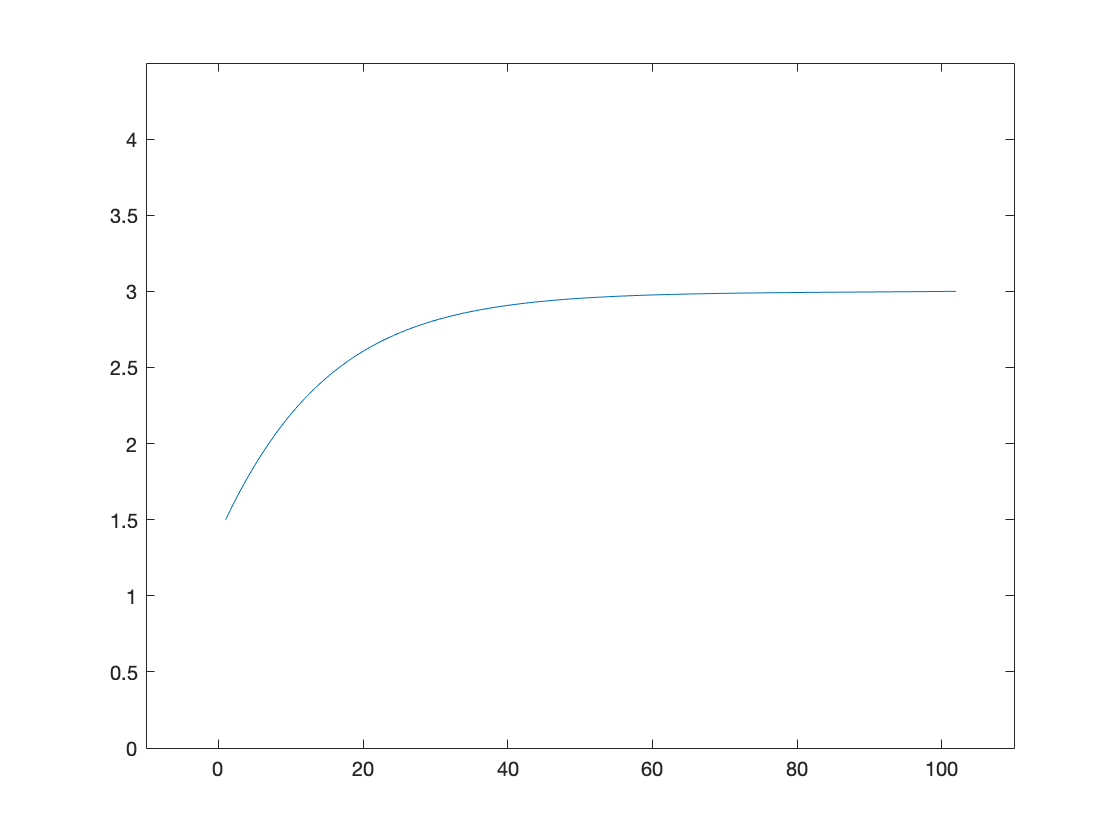
\includegraphics[scale=0.2]{ps2q3_4k1}
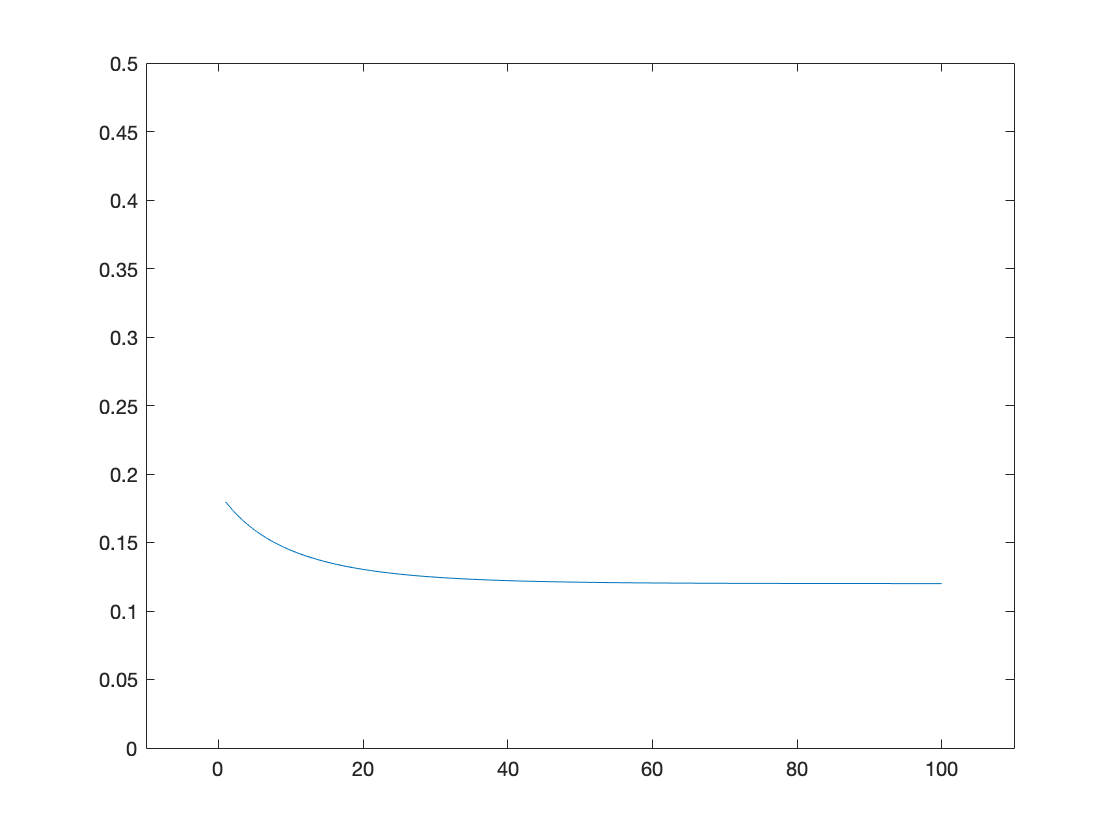
\includegraphics[scale=0.2]{ps2q3_4r_k1}
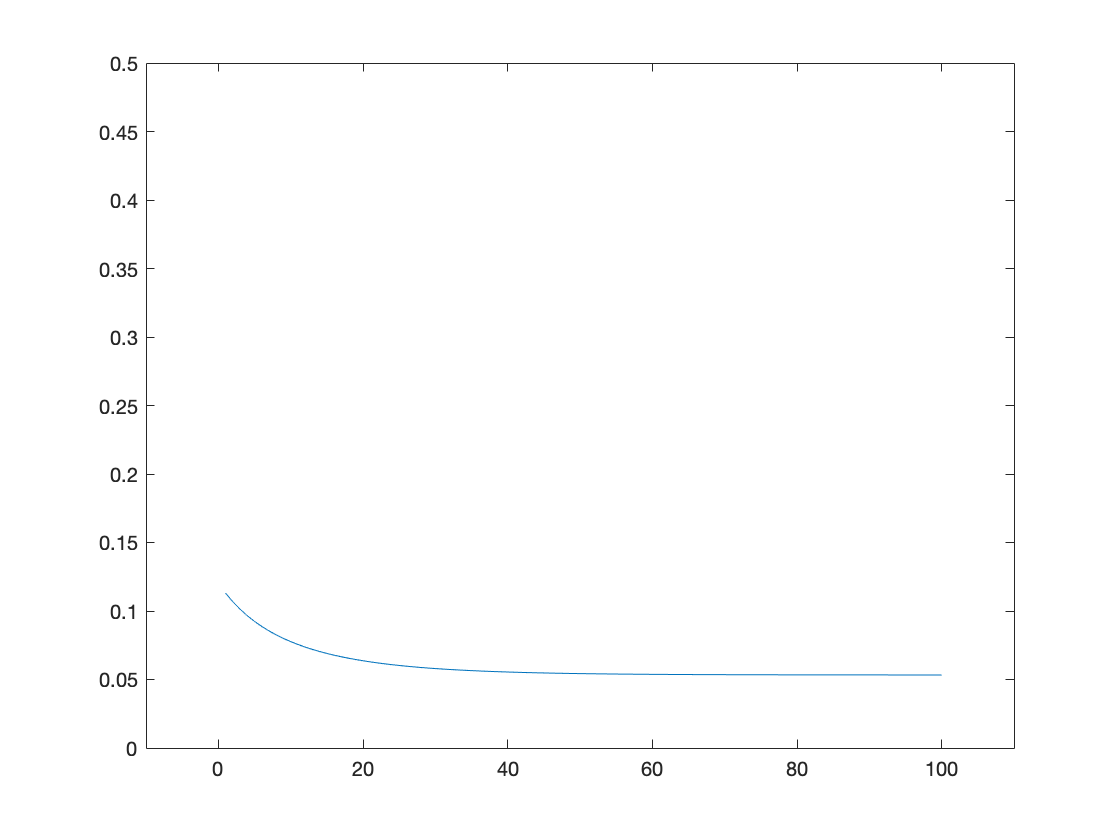
\includegraphics[scale=0.2]{ps2q3_4r_b1}
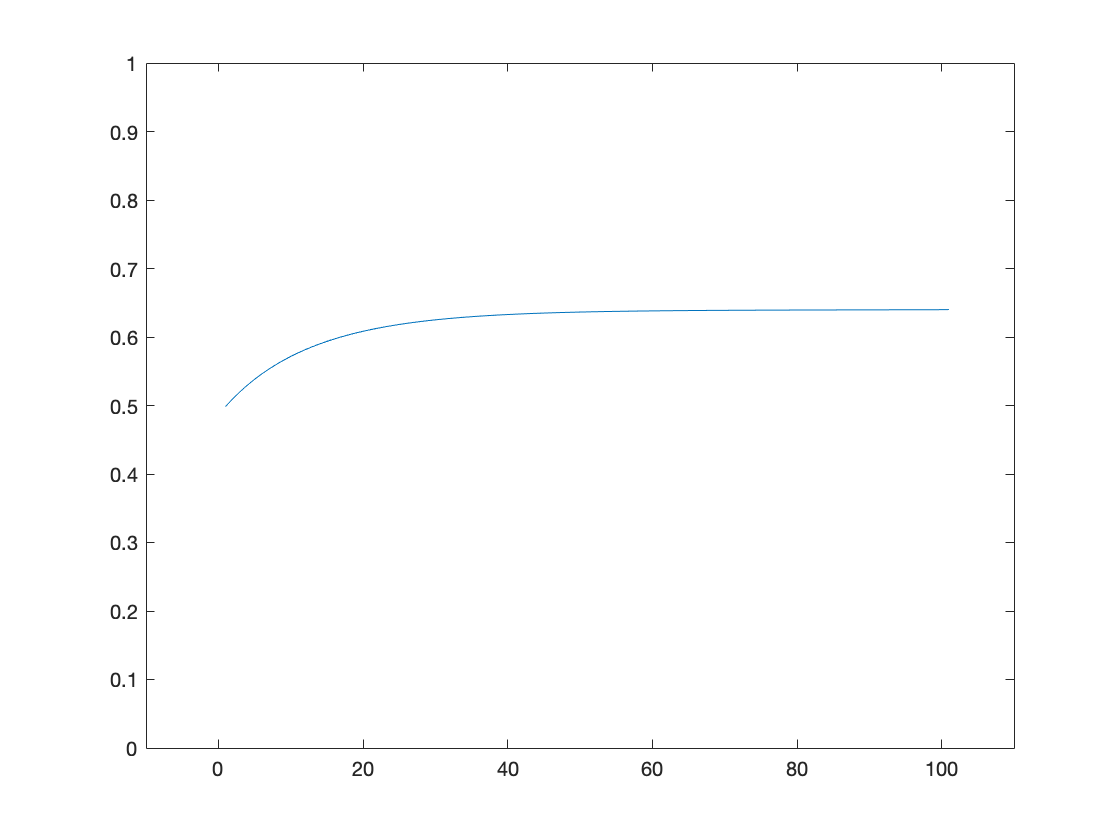
\includegraphics[scale=0.2]{ps2q3_4w1}
\caption{
Figure for $k_0 = 0.5 k_{ss}$. $k$ in the top left, $r_k$ in the top right, $r_b$ in the bottom left, $w$ in the bottom right.
}
\end{figure}
\begin{figure}
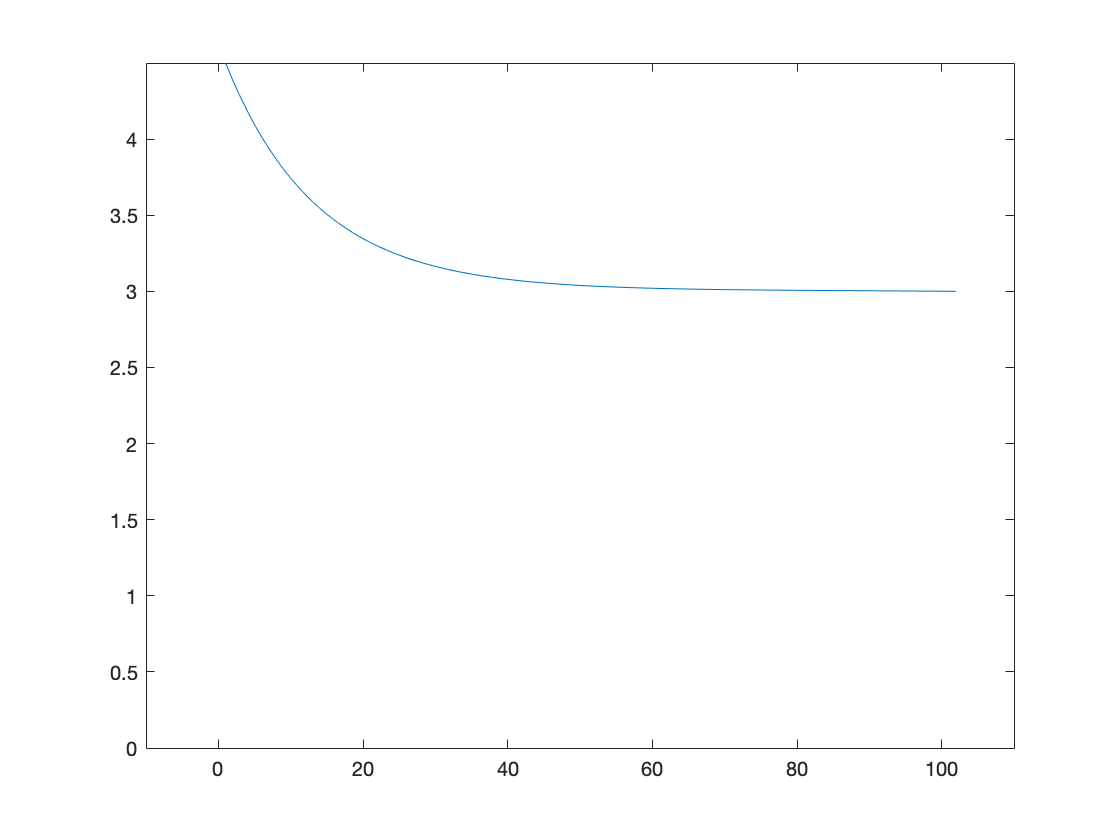
\includegraphics[scale=0.2]{ps2q3_4k2}
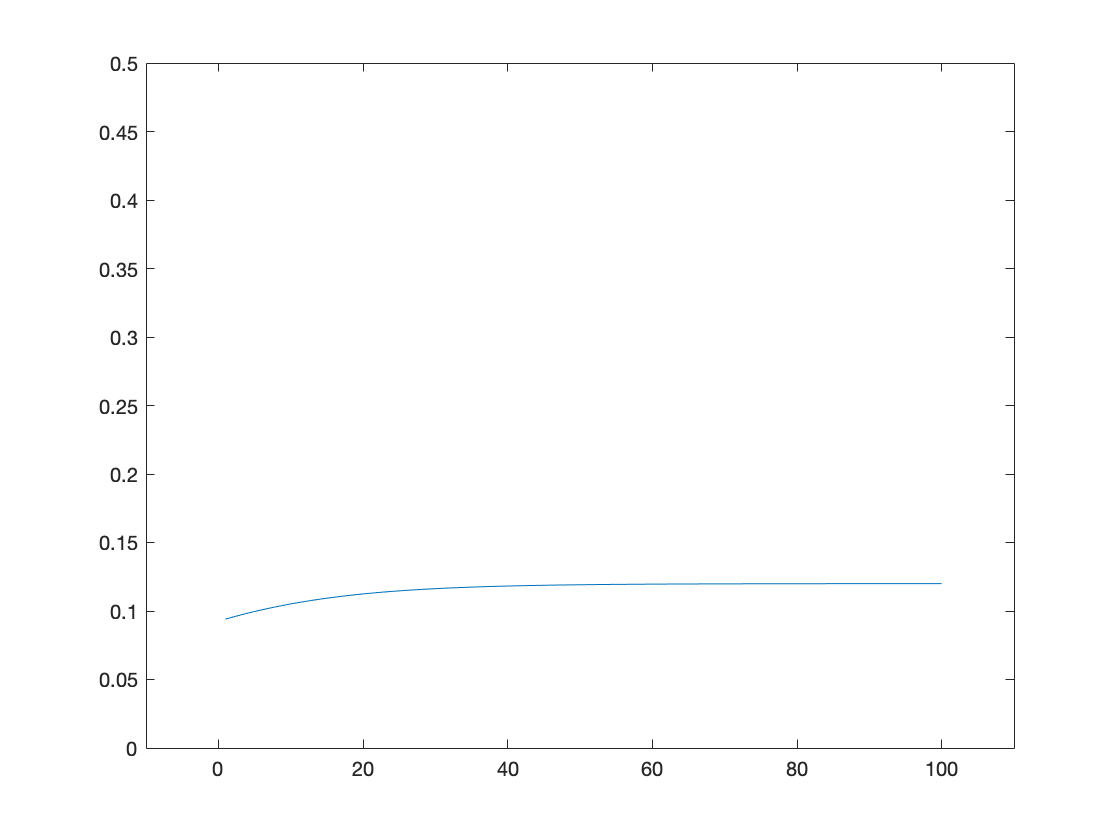
\includegraphics[scale=0.2]{ps2q3_4r_k2}
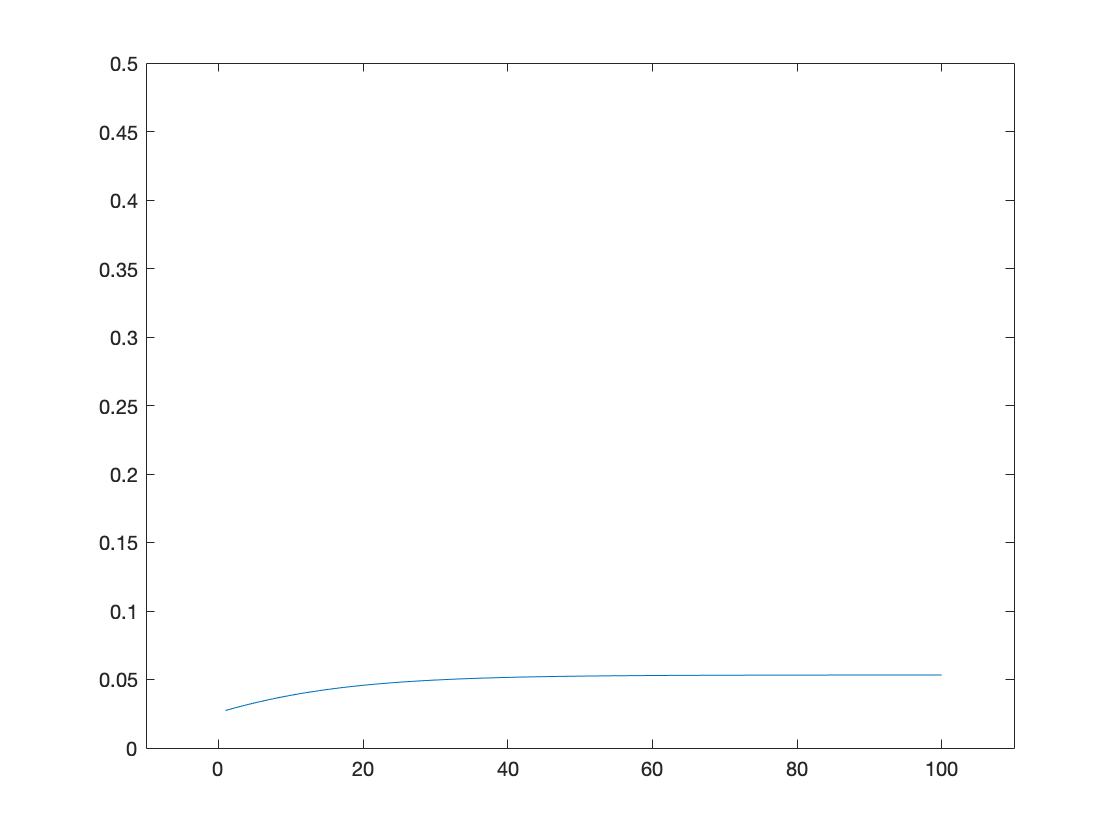
\includegraphics[scale=0.2]{ps2q3_4r_b2}
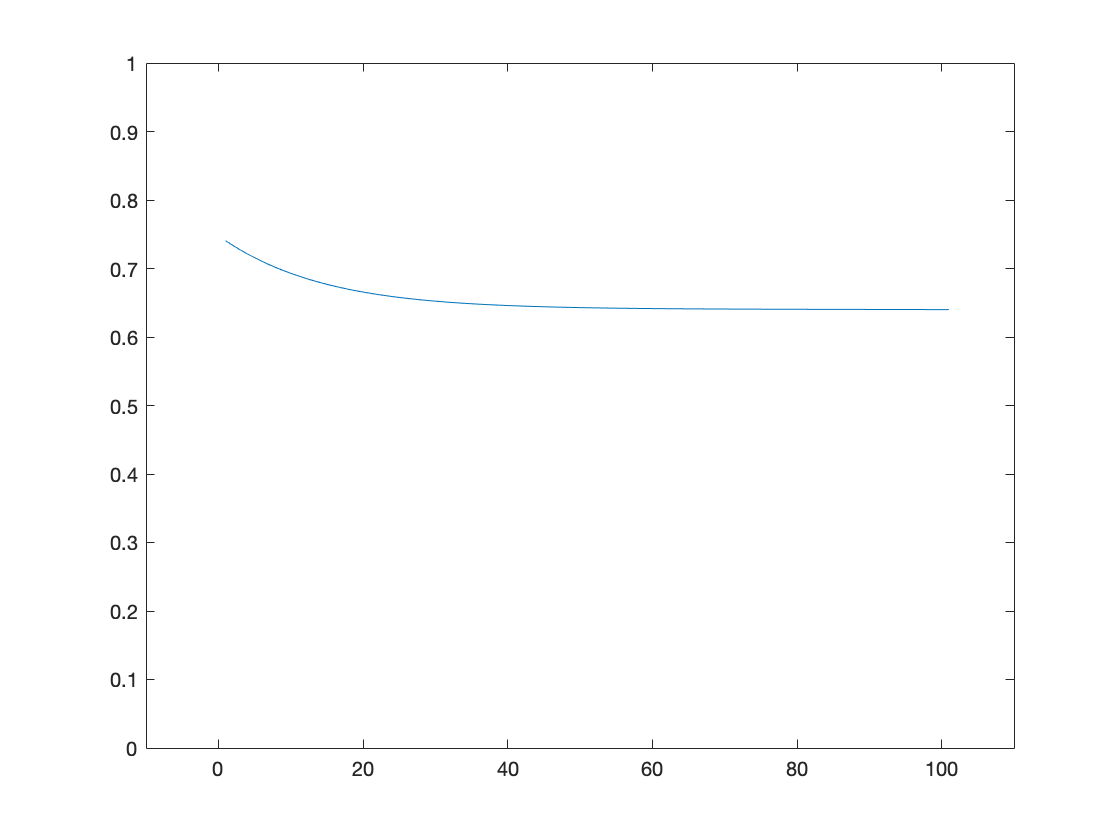
\includegraphics[scale=0.2]{ps2q3_4w2}
\caption{
Figure for $k_0 = 0.5 k_{ss}$. $k$ in the top left, $r_k$ in the top right, $r_b$ in the bottom left, $w$ in the bottom right.
}
\end{figure}
\end{document}
	% line of code telling latex that your document is ending. If you leave this out, you'll get an error
